\documentclass[12pt,a4paper]{article}

\usepackage[utf8]{inputenc}
\usepackage[T1]{fontenc}
\usepackage[brazil]{babel}
\usepackage[margin=2.5cm]{geometry}
\usepackage{graphicx}
\usepackage{booktabs}
\usepackage{longtable}
\usepackage{array}
\usepackage{tikz}
\usetikzlibrary{arrows.meta, positioning, fit}
\usepackage{hyperref}
\usepackage{caption}
\usepackage{subcaption}
\usepackage{amsmath}

\title{Análise de Resultados Iniciais\\[0.3em]
\large Otimização de Alocação de Leitos Hospitalares: Comparação entre Modelo Exato e Heurística Memética}
\author{Gustavo Ferreira Tavares\\
Curso de Graduação em Engenharia de Sistemas\\
Escola de Engenharia, Universidade Federal de Minas Gerais\\
Orientadoras: Profa. Gabriela Nunes Lopes e Profa. Luiza Bernasdes Real}
\date{Setembro de 2026}

\begin{document}

\maketitle

\section*{Introdução}

Este documento apresenta a entrega de análise de resultados iniciais do Trabalho de
Conclusão de Curso (TCC), referente ao Problema de Alocação de Leitos (PBA) em
ambiente hospitalar. O trabalho compara duas abordagens de solução para o mesmo
problema: um modelo exato de Programação Linear Inteira (PLI), resolvido via Gurobi
Optimizer, e uma heurística memética que combina Algoritmo Genético (busca
populacional global) com Busca em Vizinhança Variável — VNS (refinamento local). O
documento apresenta o enquadramento metodológico
adotado e os resultados preliminares obtidos até o momento.

\section{Metodologia}

\subsection{Classificação e Abordagem da Pesquisa}

Esta pesquisa fundamenta-se no método científico-tecnológico, caracterizando-se
como uma pesquisa aplicada e experimental: aplicada, pois tem como finalidade
resolver um problema prático de alocação de recursos hospitalares; experimental,
pois compara sistematicamente o desempenho de duas abordagens de solução sob
condições controladas e repetíveis.

Quanto à abordagem do problema, o estudo é quantitativo, pois os dois
métodos de solução são avaliados exclusivamente por meio de métricas numéricas (custo total da função objetivo, número de violações de capacidade, tempo de
processamento e número de avaliações da função objetivo) coletadas em múltiplas
execuções independentes e consolidadas estatisticamente (média e desvio padrão).
Não há coleta de dados de natureza subjetiva ou perceptiva, o que descaracteriza uma
abordagem qualitativa.

Os procedimentos técnicos adotados baseiam-se na engenharia de software
sistemática, estruturada em ciclos sucessivos de concepção, especificação,
implementação e validação para cada componente do sistema, com decisões de projeto
frequentemente revisitadas à luz de evidência empírica coletada ao longo do
desenvolvimento.

\subsection{Materiais, Ferramentas e Recursos de Engenharia}

\begin{itemize}
    \item \textbf{Ambientes de Desenvolvimento e Software:} Python 3.13, isolado em
    um ambiente virtual (\texttt{venv}) dedicado ao projeto; sistema operacional
    macOS; controle de versão via Git.

    \item \textbf{Linguagens, Frameworks e Bibliotecas:} Python como linguagem
    principal de implementação; Gurobi Optimizer (via a biblioteca
    \texttt{gurobipy}) como solver do modelo exato de Programação Linear
    Inteira; Pandas para exportação e manipulação de dados tabulares;
    Matplotlib para geração dos gráficos dos resultados.

    \item \textbf{Bases de Dados e Fontes de Informação:} por se tratarem de informações sensiveis, os dados utilizados são apenas inspirados em cenários reais, não sendo
    dados hospitalares reais. Neste trabalho, instâncias sintéticas são geradas por
    um módulo próprio (\texttt{data\_generator.py}), parametrizado para produzir
    cenários controlados e integralmente reproduzíveis (pacientes, quartos,
    especialidades clínicas, gênero e tempo de internação), em quatro escalas
    crescentes, descritas na Tabela~\ref{tab:instancias}.
\end{itemize}

\begin{table}[h]
\centering
\caption{Escalas das instâncias sintéticas utilizadas nos experimentos}
\label{tab:instancias}
\begin{tabular}{lrr}
\toprule
Instância & Quartos & Pacientes \\
\midrule
Pequeno & 10 & 100 \\
Médio & 40 & 400 \\
Grande & 160 & 1600 \\
Muito grande & 640 & 6400 \\
\bottomrule
\end{tabular}
\end{table}

\subsection{Processo de Desenvolvimento do Sistema ou Software}

O desenvolvimento seguiu um ciclo de engenharia incremental e iterativo:
cada componente do sistema foi construído, testado e refinado em ciclos sucessivos,
com ajustes de projeto (por exemplo, os pesos da função objetivo, a estratégia de
cruzamento genético e o mecanismo de escape de estagnação) sendo revisados e
retestados à medida que resultados empíricos indicavam a necessidade de mudança,
em vez de um planejamento único e definitivo antecipado no início do projeto.

O fluxo de desenvolvimento adotado foi:

\begin{center}
[ Levantamento de Requisitos ] $\rightarrow$ [ Projeto e Arquitetura ] $\rightarrow$
[ Implementação ] $\rightarrow$ [ Validação ]
\end{center}

\begin{enumerate}
    \item \textbf{Requisitos e Restrições:} formalização do Problema de Alocação de
    Leitos (PBA), conjuntos de pacientes e quartos, restrição rígida de capacidade,
    e penalidades por transferência de quarto, mistura de gênero e inadequação de
    especialidade clínica, compondo uma função objetivo ponderada.

    \item \textbf{Projeto e Arquitetura:} arquitetura orientada a objetos, com
    responsabilidades bem delimitadas por módulo (Figura~\ref{fig:arquitetura}):
    carregamento e representação da instância, avaliação de custo, modelo exato,
    heurística memética e geração de resultados.

    \item \textbf{Implementação/Construção:} codificação em Python; modelo exato
    formulado como Programação Linear Inteira e resolvido via Gurobi; heurística
    memética combinando um Algoritmo Genético (exploração global via população) com
    Busca em Vizinhança Variável (refinamento local), seguindo o paradigma de
    algoritmos meméticos da literatura.

    \item \textbf{Validação:} testes de consistência entre o cálculo
    incremental de custo (usado internamente pela heurística); comparação entre o modelo exato e a heurística nas quatro escalas de instância.
\end{enumerate}

\subsection{Procedimentos Experimentais e Coleta de Dados}

Para cada uma das quatro instâncias (Tabela~\ref{tab:instancias}), o modelo exato
(Gurobi) foi executado uma única vez, e a heurística memética foi independentemente executada
5 vezes, sem semente aleatória fixa entre execuções. Todas as execuções foram submetidas a um
teto de tempo, fixado em 5 minutos (300~s).

As variáveis observadas em cada execução foram:

\begin{itemize}
    \item \textbf{Custo total} da função objetivo (incluindo, na heurística, a
    penalidade por excesso de capacidade);
    \item \textbf{Violação de capacidade} — quantidade de leitos excedentes por
    quarto/dia, sempre nula no modelo exato (restrição rígida) e potencialmente
    positiva na heurística (restrição suave);
    \item \textbf{Tempo de processamento};
    \item \textbf{Número de avaliações da função objetivo}, métrica de esforço
    computacional adotada como padrão de comparação entre os dois métodos.
\end{itemize}

Após cada execução, os resultados são armazenados em arquivos CSV (\texttt{heuristic\_runs.csv},
\texttt{gurobi\_run.csv}, \texttt{convergence.csv}) e gráficos são gerados para representar a distribuição de custo, curva de convergência ao longo das gerações e
comparação do valor da função objetivo obtido.

\section{Resultados Iniciais e Discussão}

\subsection{Arquitetura e Implementação da Solução Inicial}

Esta primeira versão contemplando o
gerador de instâncias, o modelo exato, a heurística memética e o módulo de
geração de relatórios. A Figura~\ref{fig:arquitetura} ilustra o fluxo geral do
sistema implementado.

\begin{figure}[h]
\centering
\begin{tikzpicture}[
    node distance=0.9cm and 1.6cm,
    box/.style={rectangle, draw, rounded corners, minimum width=3.6cm, minimum height=1cm,
                align=center, fill=blue!6},
    solverbox/.style={box, fill=orange!10},
    arr/.style={-{Latex[length=2mm]}, thick}
]
\node[box] (gen) {Gerador de Instâncias\\\footnotesize\texttt{data\_generator.py}};
\node[box, below=of gen] (dm) {\texttt{DataManager}\\\footnotesize carrega \texttt{room.csv} / \texttt{patient.csv}};

\node[solverbox, below left=1.2cm and 0.2cm of dm] (gurobi) {\texttt{GurobiSolver}\\\footnotesize Modelo Exato (PLI)};
\node[solverbox, below right=1.2cm and 0.2cm of dm] (memetic) {\texttt{MemeticSolver}\\\footnotesize Algoritmo Genético + VNS};

\node[box, below=1.6cm of dm, yshift=-0.6cm] (report) {\texttt{ResultsReporter}\\\footnotesize CSVs + gráficos comparativos};

\draw[arr] (gen) -- (dm);
\draw[arr] (dm) -- (gurobi);
\draw[arr] (dm) -- (memetic);
\draw[arr] (gurobi) |- (report);
\draw[arr] (memetic) |- (report);
\end{tikzpicture}
\caption{Arquitetura geral da solução implementada: geração de instâncias,
carregamento de dados, execução do modelo exato e da heurística memética e
consolidação dos resultados.}
\label{fig:arquitetura}
\end{figure}

A heurística memética, em particular, integra os seguintes mecanismos:

\begin{itemize}
    \item Quatro vizinhanças de busca local (troca de quarto, \textit{swap} entre
    pacientes, troca parcial de quarto e \textit{swap} parcial em dias sobrepostos),
    inspiradas nas vizinhanças \textit{CR/SP/PCR/PSP} de Ceschia e Schaerf (2011),
    referência que também fundamenta a abstração de quarto/leito adotada no
    modelo;
    \item Técnica de \textit{don't-look bits} (Johnson e McGeoch) para reduzir
    drasticamente o custo computacional da busca local, evitando reavaliar
    repetidamente pacientes cujo entorno não foi alterado;
    \item Mutação com taxa disparada por estagnação: a taxa de
    mutação permanece baixa enquanto a população evolui, e passa a afetar uma
    fração garantida de pacientes quando um número configurável de gerações passa
    sem melhora, retornando à taxa normal assim que uma melhora é encontrada.
\end{itemize}

\subsection{Métricas de Desempenho e Resultados dos Testes}

A Tabela~\ref{tab:custo} consolida o custo total obtido pelo modelo exato e pela
heurística (melhor execução e média $\pm$ desvio padrão das 5 execuções
independentes) em cada instância, junto com a violação média de capacidade da
heurística (sempre nula no modelo exato, por se tratar de restrição rígida). A
Tabela~\ref{tab:esforco} consolida o tempo de processamento e o número de avaliações
da função objetivo.

\begin{table}[h]
\centering
\caption{Custo total da função objetivo e violação de capacidade}
\label{tab:custo}
\footnotesize
\begin{tabular}{lrrrr}
\toprule
Instância & Gurobi & Heur. (melhor) & Heur. (média $\pm$ dp) & Viol. cap. heur. (média) \\
\midrule
Pequeno       & 10\,225,0    & 10\,700,0    & 11\,685,0 $\pm$ 561,1     & 0,0 \\
Médio         & 39\,350,0    & 36\,425,0    & 37\,035,0 $\pm$ 670,0     & 7,2 \\
Grande        & 821\,150,0   & 114\,600,0   & 118\,025,0 $\pm$ 3\,285,7 & 52,4 \\
Muito grande  & 3\,280\,825,0 & 430\,850,0  & 441\,915,0 $\pm$ 9\,876,0 & 236,8 \\
\bottomrule
\end{tabular}
\end{table}

\begin{table}[h]
\centering
\caption{Tempo de processamento e número de avaliações da função objetivo}
\label{tab:esforco}
\footnotesize
\begin{tabular}{lrrrr}
\toprule
Instância & Tempo Gurobi (s) & Tempo Heur. (s) & Avaliações Gurobi & Avaliações Heur. (média) \\
\midrule
Pequeno       & 300 & 300 & 11\,222\,823 & 22\,296\,602 \\
Médio         & 280 & 300 & 82\,763      & 20\,898\,622 \\
Grande        & 300 & 300 & 2\,401       & 19\,528\,851 \\
Muito grande  & 310 & 300 & 0            & 16\,567\,014 \\
\bottomrule
\end{tabular}
\end{table}

\subsection{Gráficos de Convergência}

As Figuras~\ref{fig:conv-pequeno} a \ref{fig:conv-muitogrande} apresentam, para cada
instância, a curva de convergência do algoritmo memético (média das 5 execuções,
com a faixa de variação individual) ao longo das gerações, em duas visualizações
lado a lado: a versão em escala linear completa e a versão com eixo quebrado, que
isola o valor inicial (tipicamente muito mais alto) para permitir a leitura detalhada
da região onde a convergência de fato ocorre.

\begin{figure}[h]
\centering
\begin{subfigure}{0.48\textwidth}
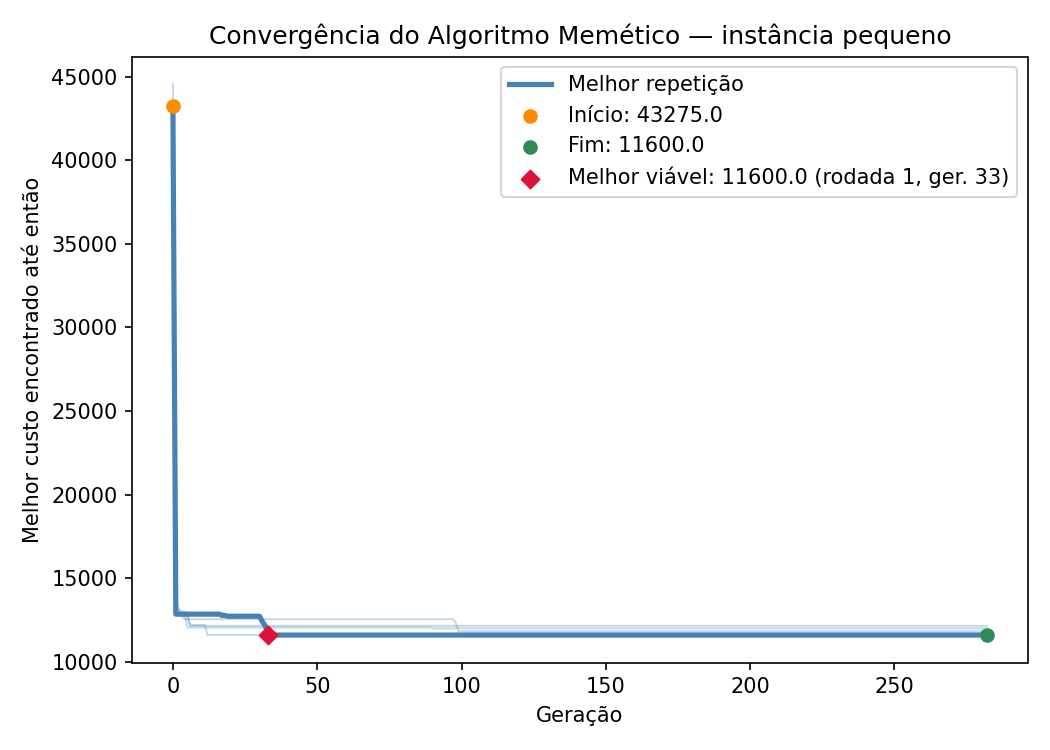
\includegraphics[width=\linewidth]{results/pequeno/convergence.png}
\end{subfigure}
\hfill
\begin{subfigure}{0.48\textwidth}
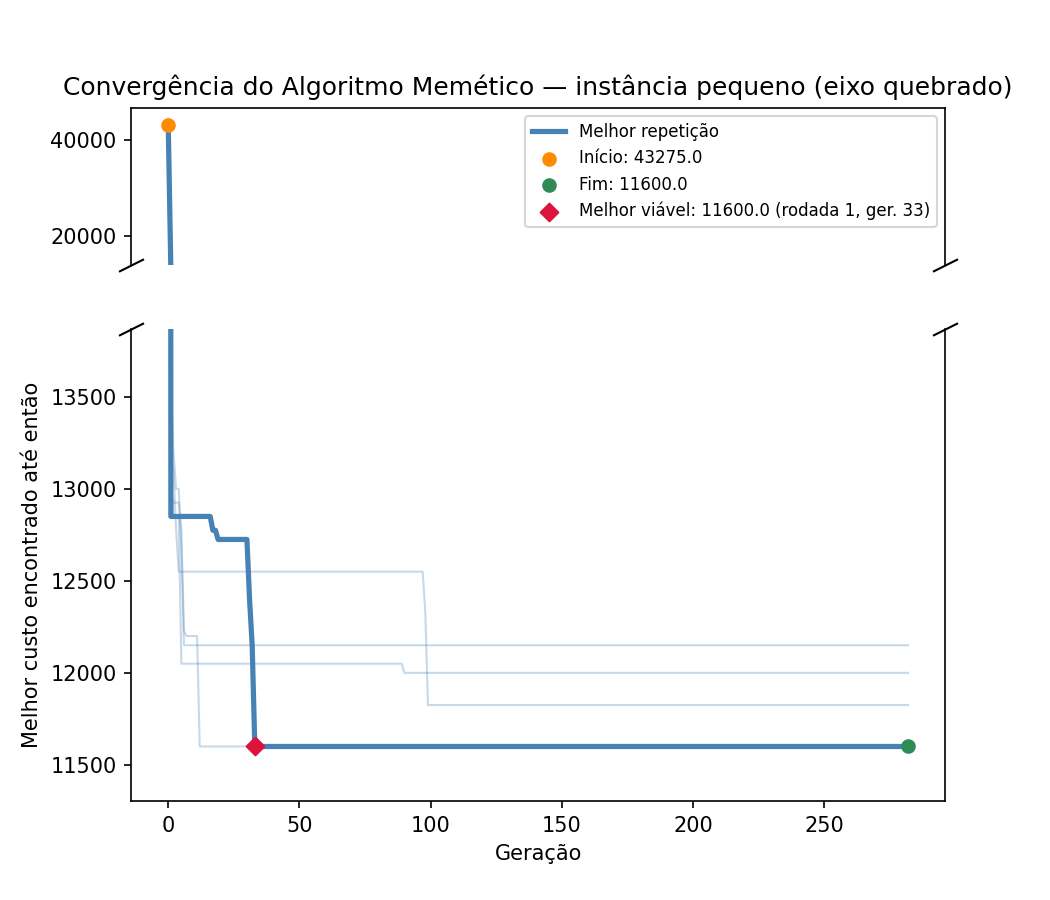
\includegraphics[width=\linewidth]{results/pequeno/convergence_broken_axis.png}
\end{subfigure}
\caption{Convergência do algoritmo memético — instância pequena.}
\label{fig:conv-pequeno}
\end{figure}

\begin{figure}[h]
\centering
\begin{subfigure}{0.48\textwidth}
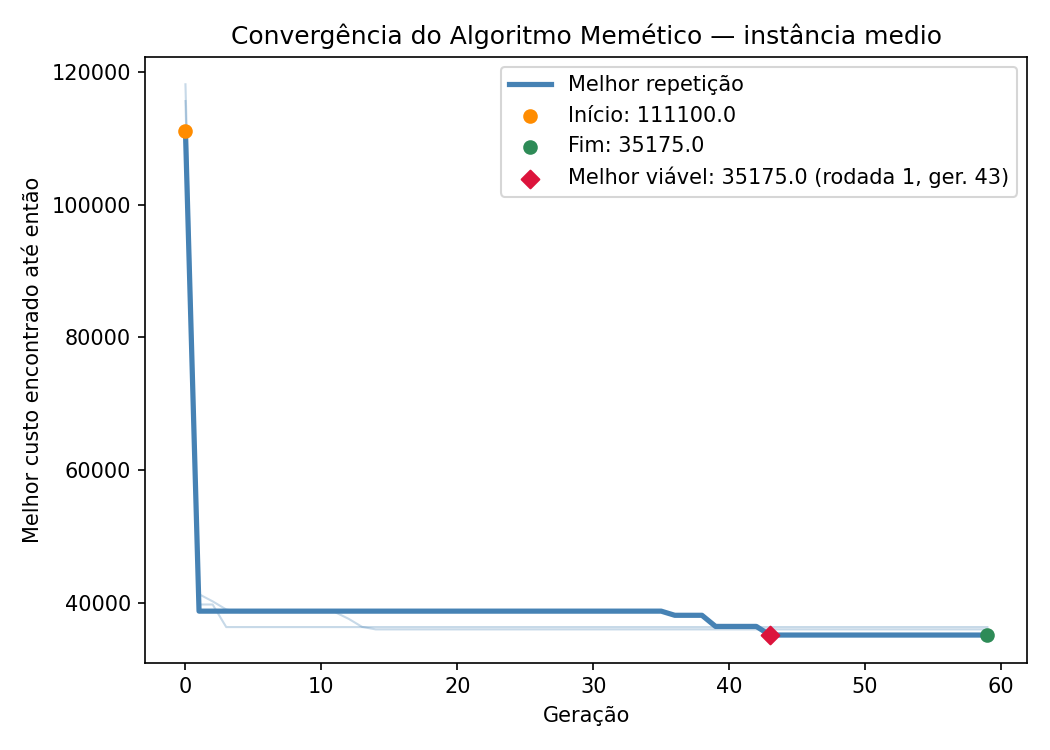
\includegraphics[width=\linewidth]{results/medio/convergence.png}
\end{subfigure}
\hfill
\begin{subfigure}{0.48\textwidth}
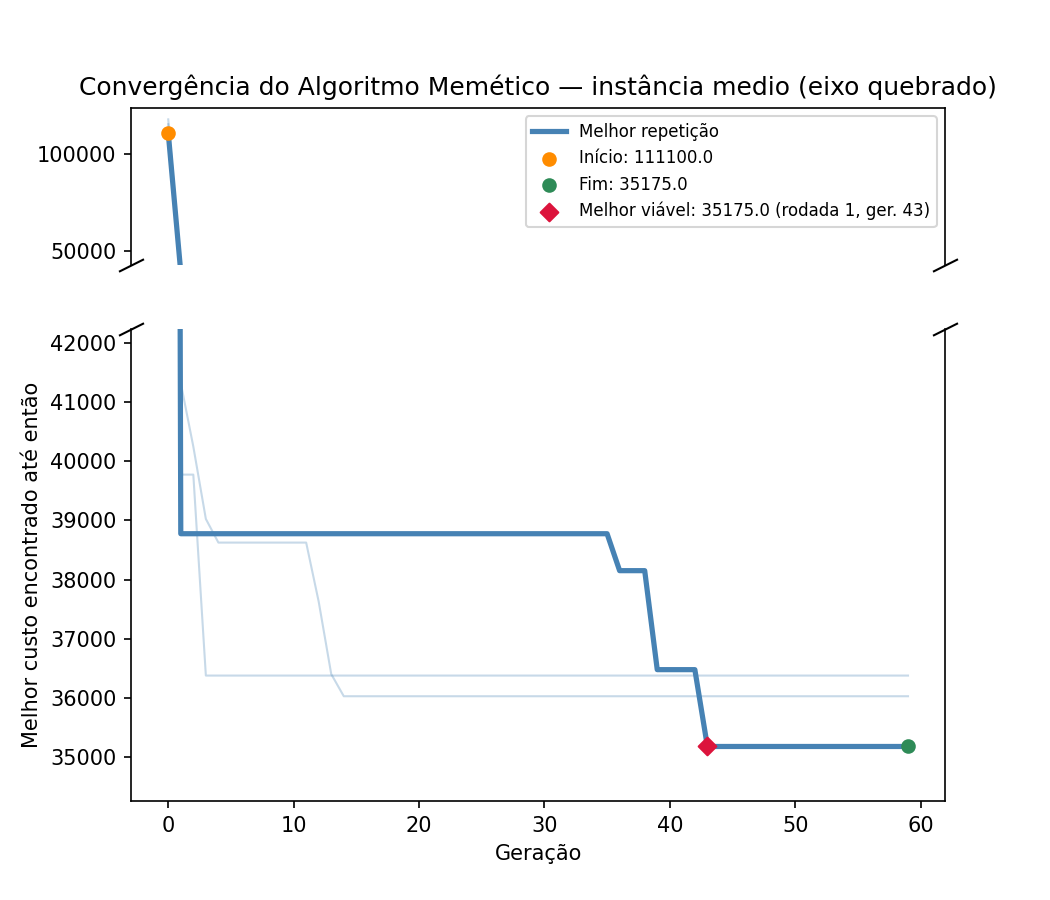
\includegraphics[width=\linewidth]{results/medio/convergence_broken_axis.png}
\end{subfigure}
\caption{Convergência do algoritmo memético — instância média.}
\label{fig:conv-medio}
\end{figure}

\begin{figure}[h]
\centering
\begin{subfigure}{0.48\textwidth}
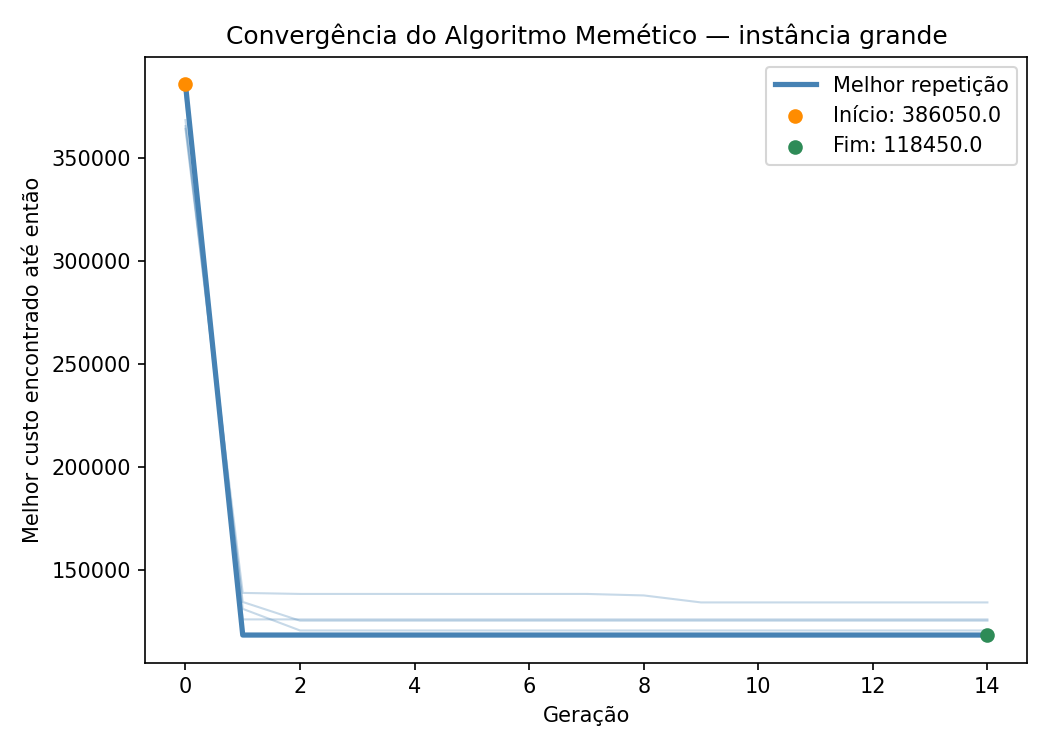
\includegraphics[width=\linewidth]{results/grande/convergence.png}
\end{subfigure}
\hfill
\begin{subfigure}{0.48\textwidth}
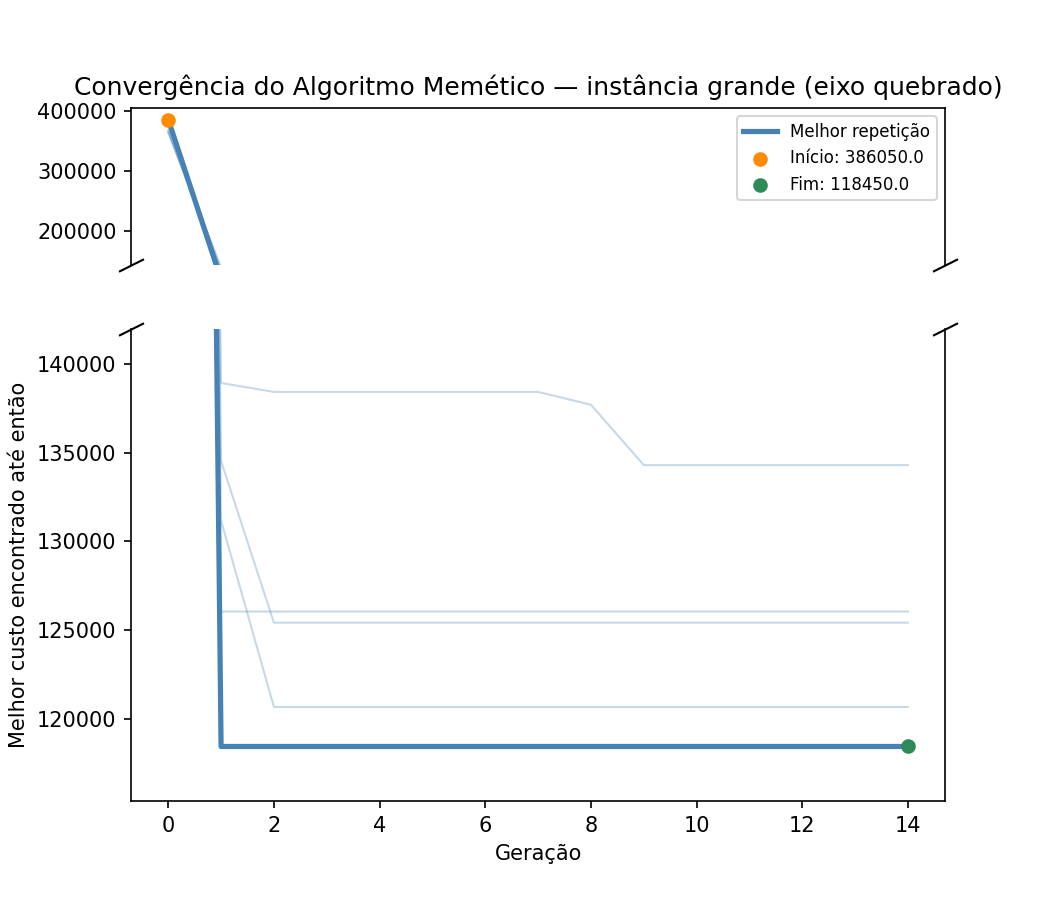
\includegraphics[width=\linewidth]{results/grande/convergence_broken_axis.png}
\end{subfigure}
\caption{Convergência do algoritmo memético — instância grande.}
\label{fig:conv-grande}
\end{figure}

\begin{figure}[h]
\centering
\begin{subfigure}{0.48\textwidth}
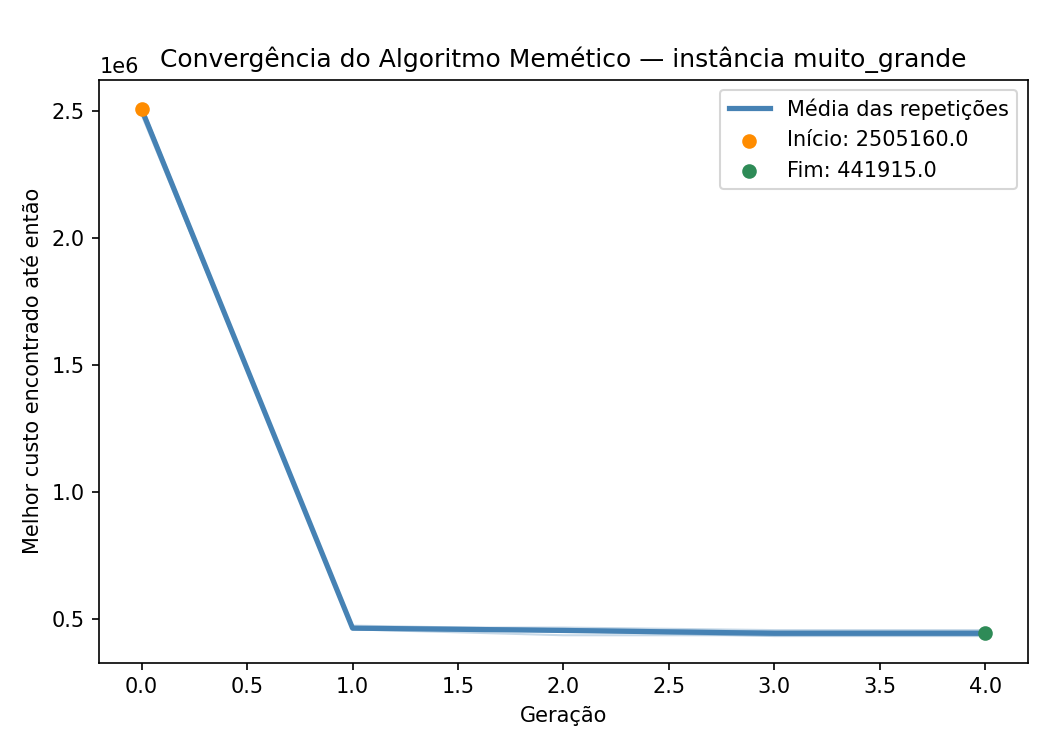
\includegraphics[width=\linewidth]{results/muito_grande/convergence.png}
\end{subfigure}
\hfill
\begin{subfigure}{0.48\textwidth}
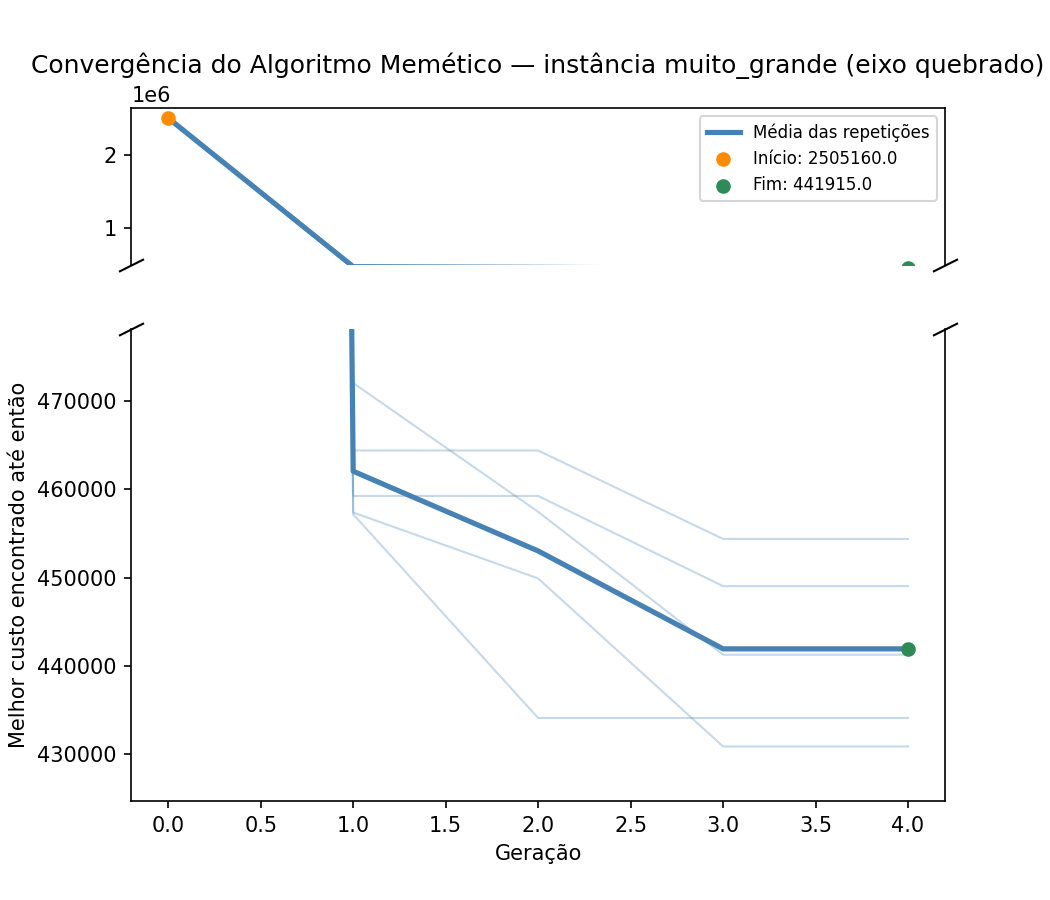
\includegraphics[width=\linewidth]{results/muito_grande/convergence_broken_axis.png}
\end{subfigure}
\caption{Convergência do algoritmo memético — instância muito grande.}
\label{fig:conv-muitogrande}
\end{figure}

\subsection{Comparação entre Gurobi e Heurística por Iteração}

A Figura~\ref{fig:gurobi-comparativo} consolida, para as quatro instâncias, o custo
total obtido pelo Gurobi e por cada uma das 5 execuções independentes da heurística,
em ordem crescente de custo.

\begin{figure}[h]
\centering
\begin{subfigure}{0.48\textwidth}
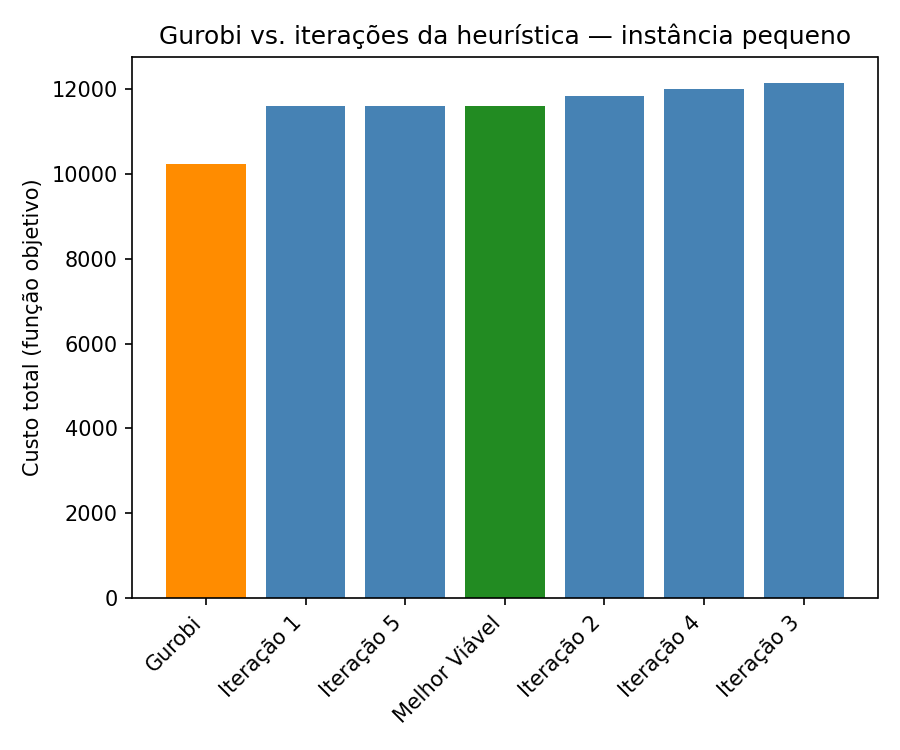
\includegraphics[width=\linewidth]{results/pequeno/gurobi_vs_iterations.png}
\caption{Pequeno}
\end{subfigure}
\hfill
\begin{subfigure}{0.48\textwidth}
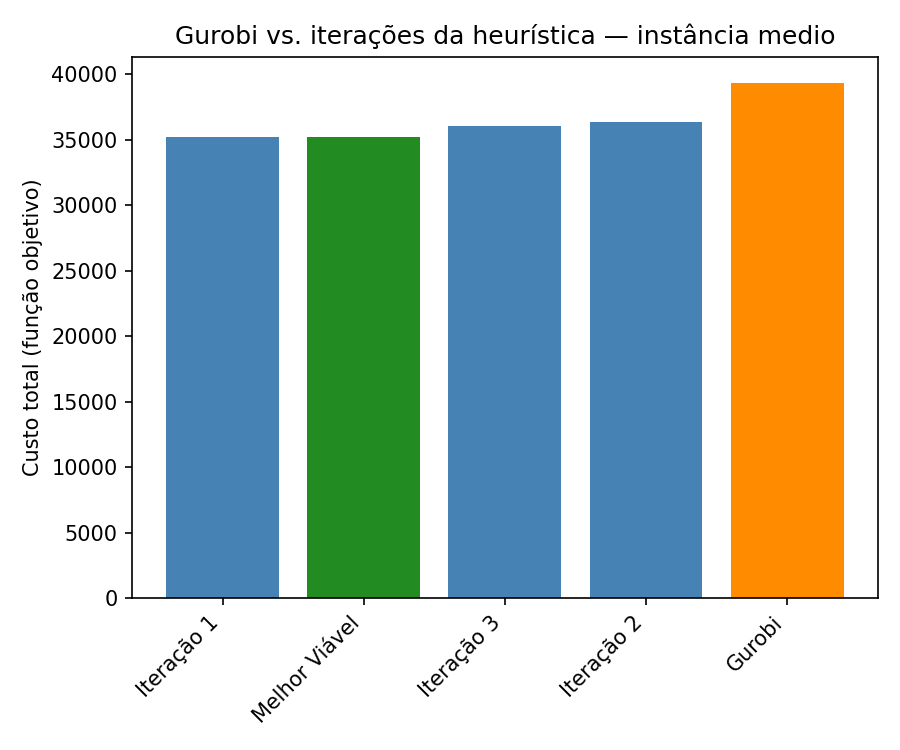
\includegraphics[width=\linewidth]{results/medio/gurobi_vs_iterations.png}
\caption{Médio}
\end{subfigure}

\vspace{0.5cm}

\begin{subfigure}{0.48\textwidth}
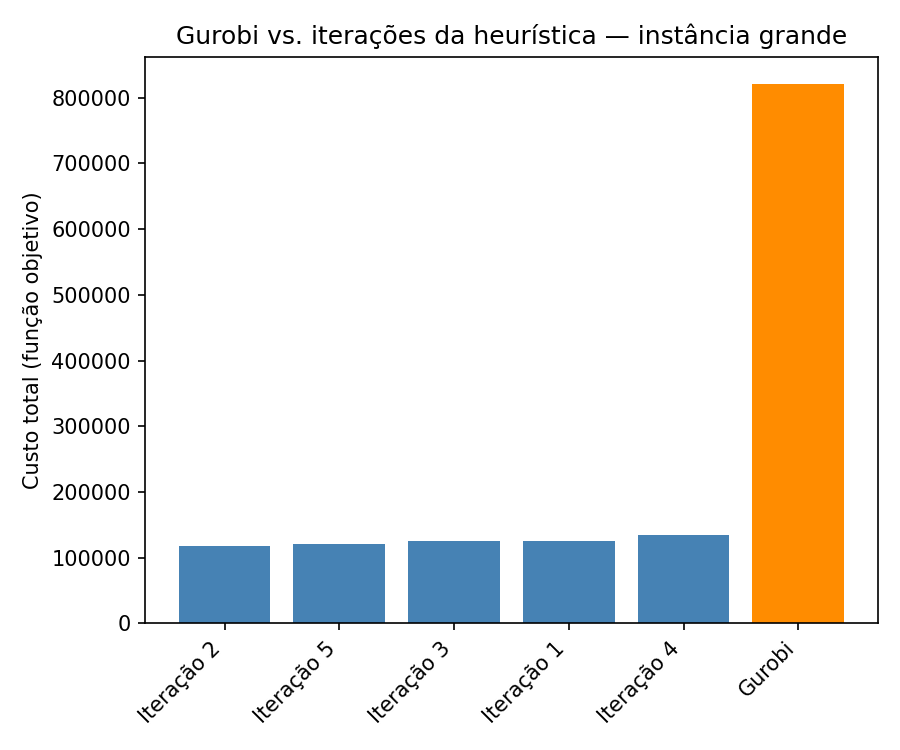
\includegraphics[width=\linewidth]{results/grande/gurobi_vs_iterations.png}
\caption{Grande}
\end{subfigure}
\hfill
\begin{subfigure}{0.48\textwidth}
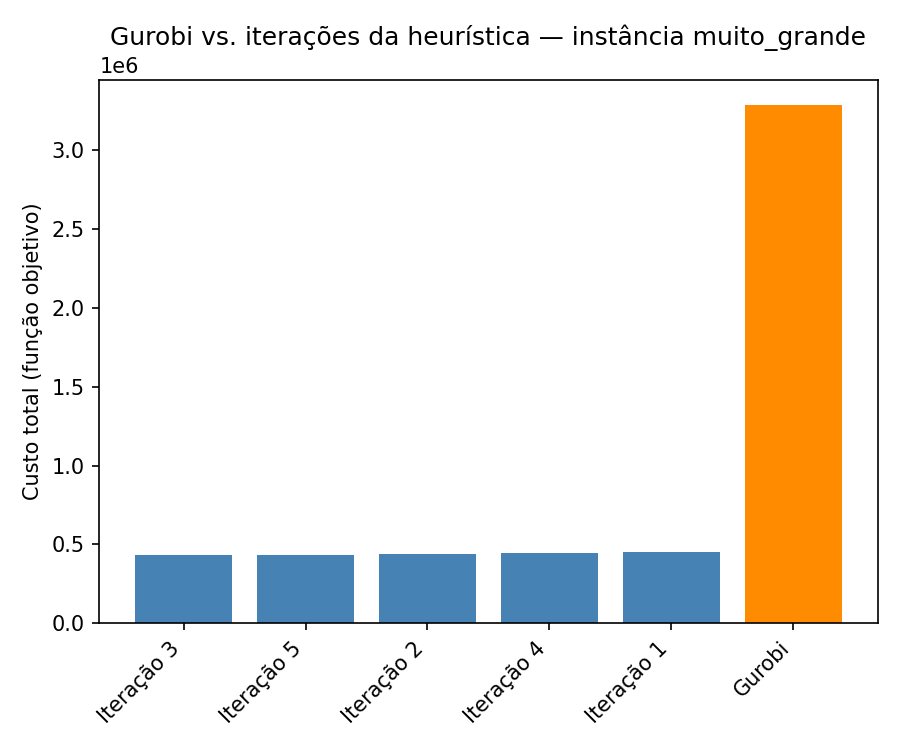
\includegraphics[width=\linewidth]{results/muito_grande/gurobi_vs_iterations.png}
\caption{Muito grande}
\end{subfigure}
\caption{Comparação entre o custo total do Gurobi e de cada execução da heurística, por instância.}
\label{fig:gurobi-comparativo}
\end{figure}

\subsection{Discussão Científica Preliminar}

Os resultados preliminares revelam um padrão consistente com a motivação central do
trabalho: o modelo exato produz soluções de excelente qualidade em
instâncias pequenas, mas seu desempenho se degrada rapidamente com o crescimento da
instância, enquanto a heurística mantém bom desempenho em todas as
escalas testadas.

Na instância \textit{pequena}, o Gurobi encontra uma solução aproximadamente 4,4\%
melhor que a melhor execução da heurística (10\,225,0 contra 10\,700,0), com ambas
as abordagens atingindo violação de capacidade nula. Já a partir da instância \textit{grande}, o quadro se inverte
drasticamente: o Gurobi entrega um custo total mais de 7 vezes maior que a
heurística (821\,150,0 contra 114\,600,0), e na instância \textit{muito grande} essa
diferença permanece na mesma ordem de grandeza (3\,280\,825,0 contra 430\,850,0). O
número de avaliações da função objetivo explica esse comportamento de forma direta:
o Gurobi realiza apenas 2\,401 iterações do método simplex na instância grande e
nenhuma iteração registrada na instância muito grande dentro dos 300~s
concedidos — um forte indício de que o \textit{solver} exato não consegue avançar de
forma significativa além da fase inicial de resolução da relaxação linear/\textit{presolve}
para modelos dessa magnitude, enquanto a heurística realiza entre 16 e 22 milhões de
avaliações no mesmo intervalo de tempo.

Um ponto que merece registro explícito é a comparabilidade da métrica de custo total
entre os dois métodos. No modelo exato, a capacidade dos quartos é uma
restrição rígida (não faz parte da função objetivo, apenas restringe o
espaço de soluções viáveis). Na heurística, por decisão de projeto, a capacidade é
tratada como restrição suave, penalizada dentro da própria função objetivo. Isso permite que a busca transite por soluções momentaneamente inviáveis em troca de
ganhos maiores em outros componentes do custo (especialidade clínica, transferências
e mistura de gênero). É esse mecanismo que explica, por exemplo, o resultado da
instância média, em que a melhor execução da heurística (36\,425,0) supera o valor
do Gurobi (39\,350,0), a solução
heurística incorre em 4 leitos de violação de capacidade (custo de penalidade de
1\,600,0), mas compensa essa violação com uma alocação de especialidade e,
sobretudo, de gênero substancialmente mais eficiente que a do Gurobi.

A literatura consultada durante o desenvolvimento (\textit{Local search and lower
bounds for the patient admission scheduling problem}, Ceschia e Schaerf, 2011) trata
exatamente dessa tensão: os próprios autores, ao descrever a busca local que
fundamenta a abstração de quarto/leito deste trabalho, penalizam o excesso de
capacidade dentro da função de custo de sua metaheurística, mesmo definindo a
capacidade como restrição rígida no modelo usado para calcular \textit{lower
bounds}, validando a decisão de projeto adotada aqui. Da mesma forma, a técnica de
\textit{don't-look bits} (consolidada por Johnson e McGeoch para busca local em
problemas de otimização combinatória) permitiu reduzir o custo de uma única chamada
de busca local em mais de uma ordem de grandeza nas maiores instâncias, sendo
determinante para viabilizar a execução da heurística dentro do teto de tempo
disponível.


\subsection{Cronograma de Atividades e Próximas Etapas}

A Tabela~\ref{tab:cronograma} apresenta o cronograma estabelecido para a conclusão
do trabalho, distribuído ao longo dos quatro meses restantes (agosto a novembro de
2026).

\begin{table}[h]
\centering
\caption{Cronograma de finalização do trabalho (TCC 2)}
\label{tab:cronograma}
\footnotesize
\begin{tabular}{p{8cm}cccc}
\toprule
Atividade / Etapa & Agosto & Setembro & Outubro & Novembro \\
\midrule
Versão do código funcionando em 80\% & X & & & \\
Versão do código 100\% finalizada & & X & & \\
Geração dos resultados, figuras de saída e tabelas de resultados & & X & & \\
Entrega do documento de análise de resultados iniciais (este documento) & & X & & \\
Entrega do ponto de controle & & X & & \\
Entrega do Capítulo de Metodologia atualizado & & X & & \\
Entrega do Capítulo de Resultados completo & & & X & \\
Entrega da Conclusão e do texto completo revisado & & & X & \\
Entrega do trabalho completo para revisão da orientadora & & & X & \\
Entrega do documento de marcação de defesa & & & X & \\
Entrega da versão final revisada para a banca & & & X & \\
Entrega do texto inicial da monografia & & & & X \\
Entrega do texto final da monografia & & & & X \\
Preparação da apresentação (slides e ensaios) & & & & X \\
Defesa das monografias & & & & X \\
\bottomrule
\end{tabular}
\end{table}

\end{document}
